%% BioMed_Central_Tex_Template_v1.06
%%                                      %
%  bmc_article.tex            ver: 1.06 %
%                                       %

%%IMPORTANT: do not delete the first line of this template
%%It must be present to enable the BMC Submission system to
%%recognise this template!!

%%% loading packages, author definitions

%\documentclass[twocolumn]{bmcart}% uncomment this for two column layout and comment line below
\documentclass{bmcart}

\usepackage{mathptmx}       % selects Times Roman as basic font
\usepackage{helvet}         % selects Helvetica as sans-serif font
\usepackage{courier}        % selects Courier as typewriter font
\usepackage{type1cm}        % activate if the above 3 fonts are not available on your system
\usepackage{makeidx}         % allows index generation
\usepackage{graphicx}        % standard LaTeX graphics tool when including figure files
\usepackage{multicol}        % used for the two-column index
\usepackage[bottom]{footmisc} % places footnotes at page bottom
\usepackage{subfig}
\usepackage{amsfonts}
\usepackage[cmex10]{amsmath}
\usepackage{float}
\usepackage[utf8]{inputenc}

\usepackage{bm} 
\usepackage{amsmath}
\usepackage{amssymb}

\usepackage{caption}

\usepackage{algpseudocode}
\usepackage{algorithm}

%%%%%%%%%%%%%%%%%%%%%%%%%%%%%%%%%%%%%%%%%%%%%%%%%
%%                                             %%
%%  If you wish to display your graphics for   %%
%%  your own use using includegraphic or       %%
%%  includegraphics, then comment out the      %%
%%  following two lines of code.               %%
%%  NB: These line *must* be included when     %%
%%  submitting to BMC.                         %%
%%  All figure files must be submitted as      %%
%%  separate graphics through the BMC          %%
%%  submission process, not included in the    %%
%%  submitted article.                         %%
%%                                             %%
%%%%%%%%%%%%%%%%%%%%%%%%%%%%%%%%%%%%%%%%%%%%%%%%%

%\def\includegraphic{}
%\def\includegraphics{}

%%% Put your definitions there:
\startlocaldefs
\endlocaldefs

%%% Begin ...
\begin{document}

%%% Start of article front matter
\begin{frontmatter}

\begin{fmbox}
\dochead{Research}

% Document information

\title{Estimation of flow trajectories in a multi-lines transportation network}

\author[
  addressref={aff1},                   
  corref={aff1},                       
  email={gguex@unil.ch}
]{\inits{G.G.}\fnm{Guillaume} \snm{Guex}}
\author[
  addressref={aff2},
  email={rloup@unil.ch}
]{\inits{R.L.}\fnm{Romain} \snm{Loup}}
\author[
addressref={aff1, aff2},
email={fbavaud@unil.ch}
]{\inits{F.B.}\fnm{François} \snm{Bavaud}}

\address[id=aff1]{%                           
  \orgdiv{Department of Language and Information Sciences},             
  \orgname{University of Lausanne},          
  \city{Lausanne},                              
  \cny{Switzerland}                                   
}
\address[id=aff2]{%
  \orgdiv{Institute of Geography and Sustainability},
  \orgname{University of Lausanne},          
  \city{Lausanne},                       
  \cny{Switzerland} 
}

\end{fmbox}

% The Abstract begins here                  

\begin{abstractbox}

\begin{abstract} % abstract
Characterizing a public transportation network, such as an urban network with multiple lines, requires the origin-destination trip counts during a given period. Yet, if automatic counting makes the embarkment (boarding) and disembarkment (alighting) counts in vehicles known, it often happens that pedestrian transfers between lines are harder to track, and require costly and invasive devices (e.g., facial recognition system) to be estimated. In this contribution, we propose a method, based on maximum entropy and involving an iterative fitting procedure, which estimates the passenger flow between origins and destinations solely based on embarkment and disembarkment flows. Moreover, this method is flexible enough to provide an adaptable framework in case additional data is known, such as attraction poles between certain points in the network, or percentages of transferring passengers between some lines. This method is tested on toy examples, as well as with the data of the public transportation network of the city of Lausanne provided by its Transportation Agency (tl), and gives convincing estimations of the transportation flow.
\end{abstract}

% Keywords begin here  

\begin{keyword}
\kwd{multiline bus network}
\kwd{origin-destination flows}
\kwd{boarding and alighting counts}
\kwd{transit flows}
\kwd{maximum entropy estimation}
\kwd{iterative proportional fitting}
\end{keyword}

% MSC classifications codes, if any
%\begin{keyword}[class=AMS]
%\kwd[Primary ]{}
%\kwd{}
%\kwd[; secondary ]{}
%\end{keyword}

\end{abstractbox}

\end{frontmatter}

% Main Body

%% --------------------------------- INTRODUCTION

\section{Introduction}
% Alternative title: Estimating transit flows from boarding and alighting counts
Transportation networks determine our mobility, require a considerable amount of planning and resources, and elicit much public hopes and critics. 
They also constitute an endless source of inspiration in formal modeling and optimization, as attested in operations research (classical optimal transportation, maximum flow problem), quantitative geography and spatial econometrics (spatial navigation, multimodality, gravity models for flows), and machine learning (recent developments in regularized optimal transportation, such as color transfer or images interpolation; see e.g. \cite{peyre2019computational}). 

This contribution addresses a straightforward, yet central question  in public transportation networks: given a network made of many train, bus, subway, or tram lines, how can one estimate the real trips made by the travelers, on the sole basis of the embarkment (boarding) counts and disembarkment (alighting) counts in each vehicle? Although estimating origin-destination flows is a much addressed issue in transportation modeling (see e.g \cite{bell1997transportation} \cite{hazelton2000estimation} \cite{ashok2002estimation} \cite{cui2006bus} and references therein), the specific problem addressed in this contribution seems, to the best of our knowledge, original. 

Pedestrian transfers of travelers between different lines here constitute the missing information, which planners traditionally try to estimate using census, or more recently with costly and invasive devices located at station, such as mobile phone tracking or facial recognition systems. In this article, we take a different approach, which is to give the best estimation of transportation trajectories without additional data, using the principle of maximum entropy. Section \ref{notforma} introduces the notations and the formalism, as well as the statement of the problem and the iterative solution method, which consist of three consecutive steps: a maximum-entropy computation of the trip distributions, obeying marginal constraints and with a given prior;  an update of the prior distribution by shrinking the components responsible for overflow; and an update of the marginal flows to avoid transfer overflow. This iterative procedure clearly evokes the EM algorithm (see e.g. \cite{dempster1977maximum}  \cite{bavaud2009information}), with the first step corresponding to the ``expectation step" and last two steps to the ``maximization step". The fist step only is required for solving the single line case (section \ref{Single line}), naturally much simpler but  yet  not trivial, and exhibiting a disembarking probability independent of the embarking stop (Markov property).  Moreover, this solution offer some flexibility, as it is possible to set a prior distribution taking into account attraction or repulsion poles among stops, and to fix hyperparameters limiting the number of transfers between lines.

In section \ref{casestudies}, we test the propose method on toy examples and the data of the public transportation network of the city of Lausanne. Toy examples offer some kind of validation, as a transportation flow can be set on toy networks and compared to the solution given by our algorithm. The real case scenario with the data from the public transportation network of the city of Lausanne shows that this method is applicable on a large transportation network and can give pertinent insights about travelers habits.


%% --------------------------------- NOTATIONS AND FORMALISM

\section{Notations and formalism}
\label{notforma}
\subsection{Lines, stops  and junctions}
\label{Lines and junctions}
Consider a \emph{transportation network} made of \emph{lines} numbered $\ell=1,\ldots, q$, of respective lengths (number of stops) $l_\ell$.  Opposite lines, that is parallel lines running in the back and forth directions are considered as distinct. 

The $l=\sum_{\ell=1}^ql_\ell$ \emph{stops} constitute the nodes of the transportation network. Each stop $i=1,\ldots,l$ belongs to a single line, and defines a unique next or forward stop $F(i)$ (unless $i$ is the line terminus) and a unique backward stop $B(i)$ (unless $i$ is the line start), both on the same line.  

Let $S_i$ denotes the \emph{set of stops which can be reached from stop $i$ outside lines connection} (with, e.g., an acceptable walking distance), excluding $i$ itself. A stop $i$ is referred to as an \emph{isolated stop} if $S_i=\emptyset$, and to as a \emph{junction} otherwise. 

\subsection{Edges, trips, and the incidence matrix}
\label{Line edges, transfer edges and trips}

Two sorts of oriented edges are involved in the transportation network: 
\begin{enumerate}
  \item[$\bullet$] \emph{intra-line edges} $(i,j)=(i,F(i))$ belonging to a single line  $\ell(i)=\ell(j)$
  \item[$\bullet$] \emph{inter-line} or \emph{transfer edges} $(i,j)$ connecting different lines $\ell(i)\neq \ell(j)$, involving walks from junction $i$ to $j\in S_i$. The \emph{set of transfer edges} is denoted by $T$.
\end{enumerate}

A \emph{$st$-trip}, noted $[s,t]$, consists of entering into the network at stop $s$, and leaving the network at $t$, by following the shortest-path (i.e. achieving the minimum distance,  minimum time, or  minimum cost), supposed unique, leading to $s$ from $t$.

The succession of edges $(i, j)$ belonging to the $st$-trip, noted $(i,j)\in [s,t]$, is unique. Define the \emph{edge-trip incidence matrix} as
\begin{equation}
\label{edgetrip}
\chi_{ij}^{st} = \begin{cases}
  1    & \text{if $(ij)\in [s,t]$}, \\
  0    & \text{otherwise}.
\end{cases}
\end{equation}

Note that we can also forbid some aberrant trips across the network, for example, trips $[s, t]$ where $(s, t)$ is a transfer edge (making this trip do not actually use the line network). The \emph{set of permitted trips} across the network is denoted by $P$, and can be defined regarding some conditions.

\vspace*{0.1cm}

\subsection{Transportation flows}
\label{Transportation flows}
Let  $x_{ij}$ count the \emph{number of travelers using edge $(i,j)$} in a given period, such as a given hour, day, week or  year.  The edge flow $x_{ij}$ is denoted by $y_{ij}$ for an intra-line edge $(i,j)$, and 
by $z_{ij}$ for a transfer edge $(i,j)$. By construction, $x_{ij}=y_{ij}+z_{ij}$, where $y_{ij}\,  z_{ij}=0$. 

\vspace*{0.1cm}


Let $a_i$, respectively $b_i$, the \emph{number of passengers embarking}, respectively \emph{disembarking} at stop $i$. By construction, 
\begin{equation}
\label{bilan1ligne}
\begin{cases}
 y_{i,F(i)}=a_i \text{\,  and } b_i=0   & \text{if $i$ is a line start}, \\
y_{B(i),i}=b_i \text{\,  and } a_i=0   & \text{if $i$ is a line terminus}, \\
 y_{i,F(i)}=y_{B(i),i}+a_i-b_i     & \text{otherwise}.
\end{cases}
\end{equation}
Also, $\mathbf{a}$ and $\mathbf{b}$ must be consistent, in the sense that $A_{B(i)}\ge B_i$, where $A_i$ (respectively $B_i$) is the \emph{cumulated number of embarked 
(resp. disembarked) passengers} on the line under consideration, recursively defined as $A_{F(i)}=A_i+a_i$ (resp. $B_{F(i)}=B_i+b_i$). Moreover,  $A_i=B_i$ at a terminal line stop $i$. This common value yields  the total number of passengers transported by the line. 



\vspace*{0.1cm}

Let the \emph{transportation flow} $n_{st}$ denotes the number of passengers following an $st$-trip, that is entering the network at $s$ and leaving the network at $t$ by using the shortest-path. One gets from (\ref{edgetrip}) 
\begin{equation}
\label{equationGG}
x_{ij}=\sum_{st}\chi_{ij}^{st}\:  n_{st}
\end{equation}
Among the passengers embarking in $i$, some transfer from another line, and some others enter into the network: 
\begin{equation}
\label{entrer}
a_i=z_{\bullet i}+n_{i\bullet}
\end{equation}
where  ``$\bullet$" denotes the summation over the replaced index, as in $n_{i\bullet}=\sum_{j=1}^l n_{ij}$. Similarly, among the passengers disembarking in $i$, some transfer to another line, and some others leave the network: 
\begin{equation}
\label{sortir}
b_i=z_{i\bullet}+n_{\bullet i}
\end{equation}
By construction
\begin{displaymath}
a_{\bullet}=b_{\bullet}=z_{\bullet\bullet}+n_{\bullet\bullet}
\end{displaymath}
where $n_{\bullet\bullet}$ counts the number of passengers, and $z_{\bullet\bullet}$ counts the number of transfers. $z_{\bullet\bullet}/n_{\bullet\bullet}$  is the average number of transfers per passenger. 

\vspace*{0.1cm}



As explained in section \ref{Lines and junctions}, transfers can only occur at junctions, that is $z_{ij}>0$ implies $(i, j) \in T$. In particular,  $z_{ii}=0$ : no traveller is supposed to disembark and re-embark later at the same stop. 


 
\subsection{Statement of the problem and solution method}
\emph{Automatic passenger counters} measure the number of passengers entering and leaving lines at each stop [Boyle, 1998], that is $\mathbf{a}$ and $\mathbf{b}$, which provide the basic raw data of the present study, kindly provided by the Lausanne Transportation Agency (tl) for the case study in section \ref{real_data}. We will suppose here that this data obeys the necessary consistency condition $a_\bullet^\ell=b_\bullet^\ell$ (where the latter quantities denote the total embarkments and disembarkments on line $\ell$), even if, in real case studies, a rescaling must usually be performed to balance in and out-flows on each lines.

Intra-line edge flows $\mathbf{Y}=(y_{ij})$ can be determined by (\ref{bilan1ligne}), but transfer edge flows $\mathbf{Z}=(z_{ij})$ are, here and typically, unknown. The objective is to estimate the $l\times l$ transportation flow matrix $\mathbf{N}=(n_{st})$. Many consistent solutions coexist in general, even for a single line with no transferts (section \ref{Single line}). This issue of incompletely observed data can be tackled by the maximum entropy formalism \cite{jaynes1957information}, which has often been the case in transportation modelling researches \cite{wilson1967statistical}  \cite{erlander1990gravity}. 



Let $f_{st}=n_{st}/n_{\bullet\bullet}$ be the \emph{distribution of $st$-trips} (empirical distribution) and let $g_{st}$ be some prior guess on its shape (theoretical distribution). 
Assuming some reasonable initial prior $g_{st}$, 
\begin{itemize}
\item[(1)] we first suppose that the empirical margins $\alpha_s=f_{s\bullet}$ and $\beta_t=f_{\bullet t}$ are known.  
Then $f_{st}$ can be determined as the maximum entropy solution (section \ref{maxenso}), i.e. as the distribution closest to $g_{st}$ in the Kullback-Leibler divergence sense under the margin constraints, to be calibrated by an iterative fitting inner loop
\item[(2)] then (section \ref{priorup}), the prior is updated to $\tilde{g}_{st}$ by shrinking, if necessary, the priors $g_{st}$, thus avoiding transfer overflow exceeding the embarking and disembarking counts at each stop. Moreover, an hyperparameter $\theta \in [0, 1]$ is used at this stage in order to control the minimum proportion of passengers entering/leaving the network at each stop.
\item[(3)] finally (section \ref{marginup}), the margins are updated to $\tilde{\alpha}_s$ and $\tilde{\beta}_t$.
\end{itemize}
With the new prior distribution $\widetilde{g}_{st}$ and the new margin distributions $\widetilde{\alpha}_s$, $\widetilde{\beta}_t$, we can iterate the 
 the above steps, until convergence. The only free parameter is $\theta$, whose effect is studied on toy examples in section \ref{toy_examples}.
 
The above iterative solution method is somewhat reminiscent of the EM algorithm. As a matter of fact, the first  step  (maximum entropy) exactly correspond to the ``expectation step" of the EM algorithm (see e.g. \cite{dempster1977maximum}  \cite{bavaud2009information}), but steps two and three, aiming at calibrating parameters $g_{st}$, $\alpha_s$ and $\beta_t$, do not follow the maximum likelihood rationale of the ``maximisation step". Pseudocode of the algorithm is shown with Algorithm \ref{algo1}.






\subsubsection{Maximum entropy estimate of $st$-trips}
\label{maxenso}
As announced,  the proportion of $st$-trips $f_{st}=n_{st}/n_{\bullet\bullet}$ (empirical distribution) will be estimated from some prior guess $g_{st}$ (theoretical distribution) and 
margin constraints $\alpha_s$ and $\beta_t$ for $f_{st}$ by maximum entropy, i.e. by 
solving the problem 
\begin{align}
	\label{constr_MaxEnt}
	\min_{\mathbf{f}\in\mathcal{F}} &\; \sum_{st}f_{st}\log \frac{f_{st}}{g_{st}}, \notag \\
	s.t. &\; \sum_t f_{st} = \alpha_s, \notag \\
	&\; \sum_s f_{st} = \beta_t.
\end{align}
The Lagragian is
\begin{equation}
	L = \sum_{st}f_{st}\log \frac{f_{st}}{g_{st}} - \sum_s \lambda_s (\alpha_s - \sum_t f_{st}) - \sum_t \mu_t (\beta_t - \sum_s f_{st}), \notag
\end{equation}
which gives, after deriving and setting to zero,
\begin{equation}
	\label{Sol}
	f_{st} = \phi_s \psi_t g_{st} \qquad \text{with } \phi_s := \exp(- 1 - \lambda_s) \text{, } \psi_t := \exp(- \mu_t).
\end{equation}
Using constraints in (\ref{constr_MaxEnt}), we find
\begin{equation}
	\label{Sol_LagMult}
	\phi_s = \frac{\alpha_s}{\sum_t \psi_t g_{st}}, \qquad \psi_t = \frac{\beta_t}{\sum_s \phi_s g_{st}}, 
\end{equation}
which yields the following \emph{iterative fitting algorithm}: starting with some $\psi^{(0)}_t > 0$, one performs the iteration
\begin{equation}
	\label{Iterative fitting}
	\phi^{(\iota)}_s = \frac{\alpha_s}{\sum_t \psi^{(\iota)}_t g_{st}}, \qquad \psi^{(\iota + 1)}_t = \frac{\beta_t}{\sum_s \phi^{(\iota)}_s g_{st}}, 
\end{equation}
until convergence to $\phi_s$ and $\psi_t$ obeying (\ref{Sol_LagMult}). 

In view of (\ref{entrer}) and (\ref{sortir}), the postulated margins must satisfy, for each isolated stop $i$
\begin{equation}
\label{ }
\alpha_i=\frac{a_i}{n_{\bullet \bullet}}\qquad\qquad \beta_i=\frac{b_i}{n_{\bullet \bullet}}
\end{equation}
permitting to determine the total flow as $n_{\bullet \bullet}=\frac{a_i}{\alpha_i}$, or  $n_{\bullet \bullet}=\frac{b_i}{\beta_i}$ for any isolated stop $i$, and thus 
the $st$-flow itself as 
\begin{equation}
	\label{flow_from_distrib}
	n_{st} = n_{\bullet \bullet} f_{st}= n_{\bullet \bullet}\phi_s \psi_t g_{st} 
\end{equation}
whose plugging into (\ref{equationGG}) yields the intra-line edge flows $\mathbf{Y}=(y_{ij})$ and the transfer edge flows $\mathbf{Z}=(z_{ij})$. Only the latter is required for subsequent algorithm steps and can be computed with 
\begin{equation}
	z_{ij} = I((i,j) \in T)\sum_{st} \chi_{ij}^{st} n_{st}
\end{equation}
where $I(.)$ denotes the 0/1 indicator function.
\subsubsection{Initialization of the prior and the margins}
The geometry of the network permits to define the set of permitted $st$-trips across the network denoted by $P$. The initial prior was chosen as the uniform distribution on admissible paths, that is as
\begin{equation*}
g_{st} = \begin{cases}
  \frac{1}{\vert P \vert}    & [s, t] \in $P$, \\
  0    & \text{otherwise}.
\end{cases}
\end{equation*}
The initial margins were chosen to initially match $g_{st}$, namely $\alpha_s=g_{s \bullet}$ and $\beta_t=g_{\bullet t}$ for all stops. However, $g_{st}$ could be chosen more carefully in case of additional data. As a matter of fact, they represent \emph{prior attractions} between nodes in equation $\ref{Sol}$, before margin correction given by $\phi_s$ and $\psi_t$ and subsequent algorithm steps. An urban planner could chose to increase or decrease some of these values in order to take into account prior knowledge on commuting habits of inhabitants.

\subsubsection{Embarkment, disembarkment constraints and hyperparameter $\theta$}
\label{constraints}
After a single iterative fitting step, the resulting transportation flow $\mathbf{N}=(n_{st})$ and transfer flow $\mathbf{Z}=(z_{ij})$ have little chance to fulfill constraints (\ref{entrer}) and (\ref{sortir}) defined by $\mathbf{a}$ and $\mathbf{b}$, and prior distributions $g_{st}$, $\alpha_s$ and $\beta_t$ must be corrected accordingly.

When $z_{\bullet i} > a_i$, or $z_{i \bullet} > b_i$, the found solution typically predict that there are more passengers entering, respectively exiting, at a stop $i$ than the actual measured quantity. One could be tempted to correct prior distributions in order to have $z_{\bullet i} = a_i$, or $z_{i \bullet} = b_i$, on every problematic nodes $i$, but the latter solution would mean that all passengers entering (resp. exiting) the line at this stop are transiting, which seems unrealistic in most real life scenarios.

We define here the hyperparameter $ \theta\in [0, 1]$ as the \emph{minimum proportion of passengers (among $a_i$ and $b_i$) entering/leaving the \textbf{network} at each stop} (in other words, not transferring), that is
\begin{equation}
n_{s\bullet}\ge \theta a_s \qquad\qquad \qquad n_{\bullet t}\ge \theta b_t
\end{equation}
or 
\begin{equation}
	z_{\bullet s} \le (1 - \theta) a_s\qquad\qquad \qquad z_{t \bullet} \le  (1 - \theta) b_t
\end{equation}
and updates of distributions will be made accordingly.

Note that, if additional data would be known, we could set a particular value of $\theta$ for every node, and differing for embarkments and disembarkments. However, without addition information, we will restrain to this simpler case. 

\subsubsection{Updating the prior distribution}
\label{priorup}
Overflow occurs in transfer edge $(i, j)$ if  $z_{i \bullet} > (1 - \theta)b_i$ or $z_{\bullet j} > (1 - \theta)a_j$. To avoid it, components $g_{st}$ of the prior distribution will be shrinked by a suitable ratio whenever edge flows $(i,j)\in [s,t]$ exhibit overflow. 
For any edge $(i, j)$, let us compute the \emph{flow ratio} $r_{ij}$ as
\begin{equation}
	r_{ij} = \max \left(1, \frac{z_{i \bullet}}{(1 - \theta)b_i}, \frac{z_{\bullet j}}{(1 - \theta)a_j} \right)\: \ge\: 1\enspace, \label{flow_ratio}
\end{equation}
where $r_{ij} > 1$ denotes an overflow through edge $(i, j)$. For a given origin-destination $[s,t]$, define the \emph{orgin-destination flow ratio} $\bar{r}_{st}$ 
as the largest $r_{ij}$ among edge flows $(i,j)\in [s,t]$, that is as 
\begin{equation}
	\label{st_flow_ratio}
	\bar{r}_{st} = \max_{ij} \chi_{ij}^{st} r_{ij}\: \ge\: 1\enspace.
\end{equation}
By construction, $\bar{r}_{st} > 1$ denotes an overflow on some transfer edge between $s$ and $t$. To adjust the flow, we shall divide the previous flow by this ratio
\begin{equation}
	\label{update_flow}
	\widetilde{n}_{st} =\frac{n_{st}}{\bar{r}_{st}}
\end{equation}
and define the new prior distribution as
\begin{equation}
	\label{update_distrib}
	\widetilde{g}_{st} = \frac{\left( \frac{\widetilde{n}_{st}}{\phi_s \psi_t} \right)}{\sum_{s',t'} \left( \frac{\widetilde{n}_{s',t'}}{\phi_{s'} \psi_{t'}} \right)}\enspace. 
\end{equation}
where $\phi_s$ and $\psi_t$ are the values (\ref{Sol_LagMult}) obtained in the previous maximum entropy step. 

\subsubsection{Updating the margin distributions}
\label{marginup}

By construction, the corrected flow $\widetilde{n}_{st}$ found in (\ref{update_flow}) now respect embarkment and disembarkment constraints. We can compute the new transfer flow on edge with
\begin{equation}
\widetilde{z}_{ij} = I((i,j) \in T)\sum_{st} \chi_{ij}^{st} \widetilde{n}_{st}
\end{equation}
and, with (\ref{entrer}) and (\ref{sortir}), updating margin distributions is straightforward 
\begin{equation}
\label{alpha_beta_update}
\widetilde{\alpha}_s = \frac{a_s - \widetilde{z}_{\bullet s}}{\sum_{s'} (a_{s'} - z_{\bullet {s'}})}   \qquad \qquad \qquad
	\widetilde{\beta}_t = \frac{b_t - \widetilde{z}_{t \bullet}}{\sum_{t'} (b_{t'} - z_{{t'} \bullet})}  \enspace. 
\end{equation}

\begin{algorithm}[h]
	\caption{Compute the transportation flow matrix $\mathbf{N} = (n_{st})$ knowing the edge-trip incidence matrix $\bm{\chi} = (\chi_{ij}^{st})$, the set of transfer edges $T$, the set of permitted trips $P$, the embarking flow $\mathbf{a}$, the disambarking flow $\mathbf{b}$, the index of an isolated source node $\tilde{s}$, and the minimum proportion of passengers entering/leaving the network $\theta$.}
	\label{algo1}
	\begin{algorithmic}[1]
		\State $g_{st} \leftarrow I([s, t] \in P) / \vert P \vert, \; \forall s,t$ \Comment{{\footnotesize Initialize the prior distribution}}
		
		\State $\alpha_s \leftarrow g_{s\bullet}, \; \forall s$ \Comment{{\footnotesize Initialize the network ingoing distribution}}
		
		\State $\beta_t \leftarrow g_{\bullet t}, \; \forall t$ \Comment{{\footnotesize Initialize the network outgoing distribution}}
		
		\State $\epsilon \leftarrow 10^{-40}$ \Comment{{\footnotesize Fix a small quantity}}
		
		\While{$\mathbf{N} = (n_{st})$ has not converge} \Comment{{\footnotesize Main loop}}
		
		\State $\psi_t \leftarrow 1, \; \forall t$
		
		\While{$\bm{\psi} = (\psi_t)$ has not converge} \Comment{{\footnotesize Iterative fitting loop}}
		
		\State $\phi_s \leftarrow \alpha_s / (\sum_t \psi_t g_{st} + \epsilon), \; \forall s$
		\State $\psi_t \leftarrow \beta_t / (\sum_s \phi_s g_{st} + \epsilon), \; \forall t$
		
		\EndWhile
		
		\State $n_{st} \leftarrow \frac{a_{\tilde{s}}}{\alpha_{\tilde{s}}} \phi_s \psi_t g_{st}, \; \forall s,t$ \Comment{{\footnotesize Compute the transportation flow}}
		
		\State $z_{ij} \leftarrow I((i,j) \in T)\sum_{st} \chi_{ij}^{st} n_{st}, \; \forall i,j$
		
		\State $r_{ij} \leftarrow \max \left(1, \frac{z_{i \bullet}}{(1 - \theta)b_i}, \frac{z_{\bullet j}}{(1 - \theta)a_j} \right), \; \forall i,j$
		
		\State $\bar{r}_{st} \leftarrow \max_{ij} \chi_{ij}^{st} r_{ij}, \; \forall s,t$
		
		\State $\widetilde{n}_{st} \leftarrow \frac{n_{st}}{\bar{r}_{st}}, \; \forall s,t$
		
		\State $\widetilde{g}_{st} \leftarrow \frac{\left( \frac{\widetilde{n}_{st}}{\phi_s \psi_t + \epsilon} \right)}{\sum_{s',t'} \left( \frac{\widetilde{n}_{s't'}}{\phi_{s'} \psi_{t'} + \epsilon} \right) + \epsilon}, \; \forall s,t$ \Comment{{\footnotesize Update the prior distribution}}
		
		\State $\widetilde{z}_{ij} \leftarrow I((i,j) \in T)\sum_{st} \chi_{ij}^{st} \widetilde{n}_{st}, \; \forall i,j$
		
		\State $\alpha_s \leftarrow \frac{a_s - \widetilde{z}_{\bullet s}}{\sum_{s'}(a_{s'} - \widetilde{z}_{\bullet {s'}})}, \; \forall s$ \Comment{{\footnotesize Update the network ingoing distribution}}
		
		\State $\beta_t \leftarrow \frac{b_t - \widetilde{z}_{t \bullet}}{\sum_{t'} (b_{t'} - \widetilde{z}_{{t'} \bullet})}, \; \forall t$ \Comment{{\footnotesize Update the network outgoing distribution}}
		
		\EndWhile
		\State \Return $\mathbf{N} = (n_{st})$
	\end{algorithmic}
\end{algorithm}


\subsection{Markov property for a single line}
\label{Single line}
A ``network" made of a single line contains no transfers, and flow estimates can be obtained at once by the maximum entropy step only.


Let  $i=1,\ldots, l$ enumerate the bus stops in increasing order,  i.e. $F(i)=i+1$. The initial prior is simply $g_{st}=c\; I(s<t)$ and captures solely the unidirectional nature of trips, where $c=\frac{1}{(l-1)(l-2)}$.   The margins of the empirical distribution $f_{st}$, as well as the total flow, are here known : 
\begin{displaymath}
\alpha_s=\frac{a_s}{a_\bullet}\qquad\qquad\qquad \beta_t=\frac{b_t}{b_\bullet}\qquad\qquad\qquad n_{\bullet\bullet}=a_{\bullet}=b_\bullet\enspace. 
\end{displaymath}
Following  (\ref{Sol}) maximum entropy flows are of the form
\begin{equation}
\label{nosignle}
n_{st}= n_{\bullet\bullet}\,  c\, I(s<t)\, \phi_s\,  \psi_t 
\end{equation}
where (setting $\Psi_s:=\sum_{t>s}\psi_t$ and $\Phi_t:=\sum_{s<t}c\phi_s$) the constraints (\ref{Sol_LagMult}) equivalently read
\begin{equation}
\label{dis embarking constraints}
\phi_s=\frac{\alpha_s}{c\, \sum_{t>s}\psi_t}=\frac{a_s}{n_{\bullet\bullet}\,  c\, \Psi_s}
\qquad\qquad\qquad
\psi_t=\frac{\beta_t}{c\, \sum_{s<t}\phi_s}=\frac{b_t}{n_{\bullet\bullet}\, c\, \Phi_t}
\end{equation}
to be solved by iterative fitting. 

Interestingly enough, the form (\ref{nosignle}) for the flows is reminiscent of the {\em gravity flows} of quantitative Geography \cite{wilson1967statistical}  \cite{erlander1990gravity} \cite{bavaud2002quasi} \cite{Thomas-Agnan2021}, where 
$\phi_s$ is the {\em push factor}, $\psi_t$ is the {\em pull factor}, and $I(s<t)$ the {\em distance deterrence function}. Yet, instead of  
being symmetric in $s,t$ and decreasing with the distance $|s-t|$, the distance deterrence function is here asymmetric due to the line orientation, but otherwise constant. 

This constancy entails the following Markovian behaviour for flows: let $m_{st}$ be the number of travelers embarking at stop $s$ and still inside the bus at stop $t>s$, and let $\rho_{st}$ the probability that travelers embarking at $s$ will disembark at $t$. By (\ref{nosignle}), 
\begin{displaymath}
m_{st}=\sum_{u\ge t}n_{su}=n_{\bullet\bullet}\, c\, \phi_s  \sum_{u\ge t} I(s<u)\, \psi_u =n_{\bullet\bullet}\, c\,  \phi_s (\psi_t+\Psi_t) 
\end{displaymath}
The empirical estimate of $\rho_{st}$ is given by the proportion, among the travelers embarking at $s$ and 
 still present at $t>s$,  of travelers disembarking at $t$, that is 
\begin{displaymath}
\rho_{st}=\frac{n_{st}}{m_{st}}=\frac{n_{\bullet\bullet}\, c\,  \phi_s\,   \psi_t}{n_{\bullet\bullet}\, c\,  \phi_s (\psi_t+\Psi_t)}=\frac{\psi_t}{\psi_t+\Psi_t}\le 1 
\end{displaymath}
which depends on $t$ only: it appears that the disembarkment probability $\rho_t=\frac{\psi_t}{\psi_t+\Psi_t}$ at $t$ is {\em independent} of the embarkment stop $s$. Said otherwise, a traveler embarking at any stop $s$ (and thus necessarily in the bus at $F(s)=s+1$) experiences the {\em same disembarkment probability} at each further stop $t>s$. 


This Markov property, enjoyed by maximum-entropic flows, contrasts other possible solutions, such as  the ``first in, first out" (FIFO) flows (homogenizing the 
traveled distances among users) or the ``last in, first out" (LIFO) flows (tending to generate maximally  contrasted traveled distances).

 
%% --------------------------------- CASE STUDIES

\section{Case Studies}
\label{casestudies}

Case studies are divided in two sections. In the first section, we test the algorithm on toy examples, which are artificial networks where the transportation flow $n_{st}$ is randomly drawn. These examples enable some kind of validation of the algorithm, as the "real" transportation flow is known and can be compared to solutions given by our method. This setup differs from the second section, which is dedicated to applying the algorithm to the real case of the public transportation network of the city of Lausanne (tl), where embankment and disembarkment flows are measured but the real transportation flow is unknown. This second case study shows that the algorithm is applicable on large, real datasets and can gives insights about passengers probable routes in the network.

\subsection{Error measurements}
\label{error_measures}

In all case studies, we obtain a estimation of the transportation flow with the algorithm, noted $\mathbf{N} = (n_{st})$, starting from the real embarkment flow $\mathbf{a}_\text{ref}$ and disembarkment flow $\mathbf{b}_\text{ref}$. In toy examples, we also have access to the real transportation flow $\mathbf{N}_\text{ref}$. 
There are two types of dissimilarity measures between the data and the solution proposed by the algorithm: (1) if we have access to $\mathbf{N}_\text{ref}$, how much $\mathbf{N}$ differs from it, and (2) how well constraints defined by $\mathbf{a}_\text{ref}$ and $\mathbf{b}_\text{ref}$ are respected. The first dissimilarity is measured through the \emph{mean transportation error}, denoted by $\text{MTE}(\mathbf{N})$, and computed with
\begin{equation}
	\text{MTE}(\mathbf{N}) = \sum_{st} \frac{n^\text{ref}_{st}}{n^\text{ref}_{\bullet \bullet}} \frac{\lvert n_{st} - n^\text{ref}_{st}\lvert}{n^\text{ref}_{st}} = \frac{\sum_{st} \lvert n_{st} - n^\text{ref}_{st}\lvert}{n^\text{ref}_{\bullet \bullet}} 
	\label{MTE}
\end{equation} 
and the second one with the \emph{mean margin error}, noted $\text{MME}(\mathbf{N})$, obtained with
\begin{align}
	\text{MME}(\mathbf{N}) &= \frac{1}{2} \sum_{i} \frac{a^\text{ref}_i}{a^\text{ref}_\bullet} \frac{\lvert z_{\bullet i} + n_{i \bullet} - a^\text{ref}_i \lvert}{a^\text{ref}_i} + \frac{1}{2} \sum_{i} \frac{b^\text{ref}_i}{b^\text{ref}_\bullet} \frac{\lvert z_{i \bullet} + n_{\bullet i} - b^\text{ref}_i \lvert}{a^\text{ref}_i} \notag \\
	&= \frac{\sum_i (\lvert z_{\bullet i} + n_{i \bullet} - a^\text{ref}_i \lvert + \lvert z_{i \bullet} + n_{\bullet i} - b^\text{ref}_i \lvert)}{2n^\text{ref}_{\bullet \bullet}}
	\label{MME}
\end{align} 
where $z_{ij} = I((i,j) \in T)\sum_{st} \chi_{ij}^{st} n_{st}$ is the flow on transfer edges $T$. Both errors can be interpreted as a weighted mean of a percentage of error.

Note that, by construction, the MME should be null when the algorithm converges. However, it can be informative to track down this error along iterations and, in some practical cases where margin constraints are impossible to fulfill, the algorithm convergence criterion is reached with MME $> 0$.

\subsection{Toy Examples}
\label{toy_examples}

\subsubsection{Construction}
\label{example_construction}

All constructed toy examples are built following the same approach, which aims at being simple but somewhat realistic. We fix a number of \emph{line tours} $p \geq 2$, each of which is constituted of a forward line and a backward line, for a total of $q = 2p$ lines. Every line has a starting and ending node, which are isolated node, and posses $p-1$ intermediary nodes which allows transfers to the other tour lines, giving a total of $n = 2p(p + 1)$ nodes in the network. Examples of these toy networks can be found in Figure \ref{toy_example_plots}.

\begin{figure}[h]
	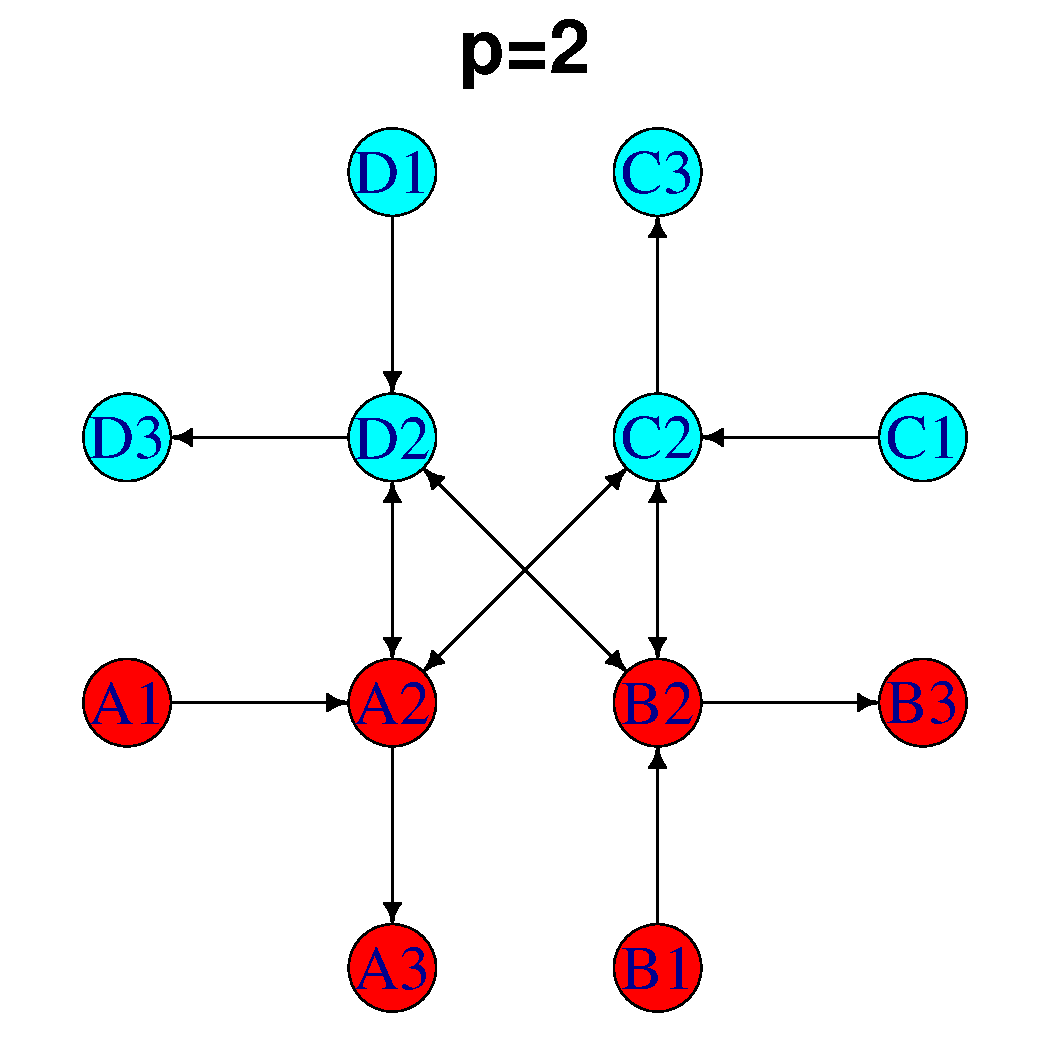
\includegraphics[width=0.3\textwidth]{fig/toy_2_display.pdf}
	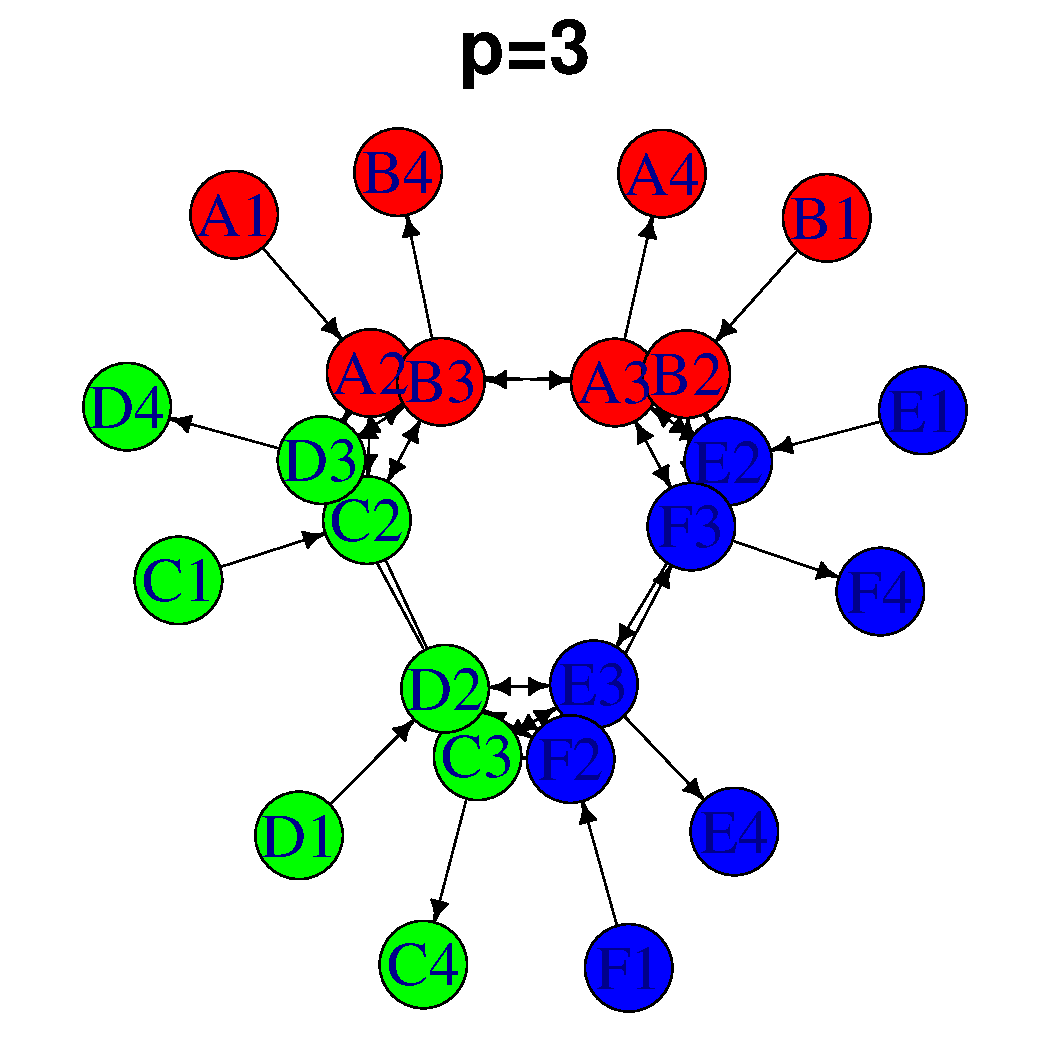
\includegraphics[width=0.3\textwidth]{fig/toy_3_display.pdf}
	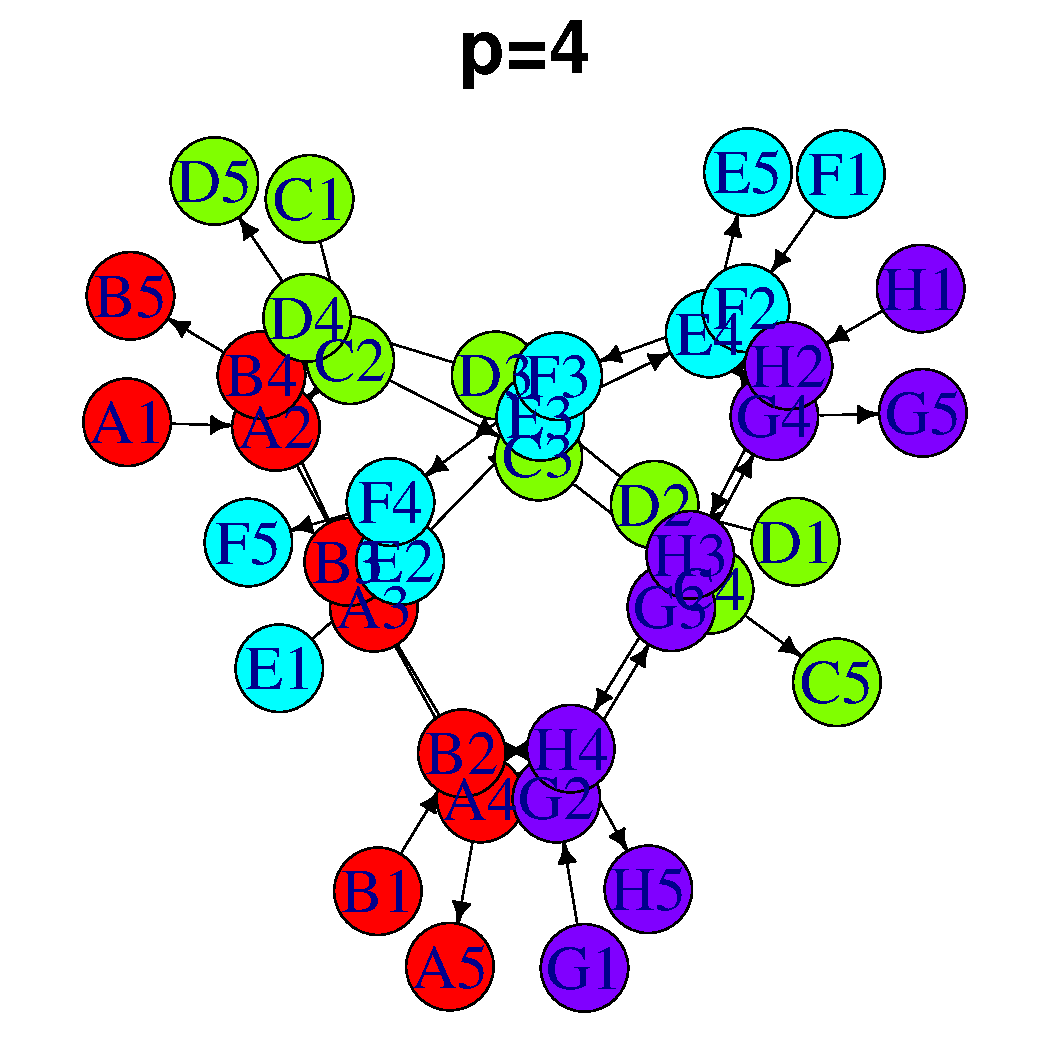
\includegraphics[width=0.3\textwidth]{fig/toy_4_display.pdf}
	\caption{3 toy examples, with the number of tours $p \in \{2,3,4\}$. Tours are displayed in the same color, line have a unique letter, and each stop a unique combination of a letter and a number. Clusters of nodes represent positions where transfer between tours are possible.}
	\label{toy_example_plots}
\end{figure}

In order to be realistic, permitted $st$-trips set $P$ is constructed considering all shortest-path between pair of nodes, excluding :
\begin{itemize}
\item $s$ and $t$ that are on the same line but with $t$ preceding $s$ in the line order.
\item $s$ and $t$ that are on the same tour but opposite line.
\item $s$ and $t$ whose shortest-path starts with a transfer edge, ends with a transfer edge, or possesses two (or more) consecutive transfer edges.
\end{itemize}

A transportation flow $\mathbf{N}_\text{ref} = (n^\text{ref}_{st})$ is drawn by setting a fixed number of passengers $n^\text{ref}_{\bullet \bullet}$, and each passenger is assigned randomly to a $(s, t)$ pair drawn uniformly among $P$. From this reference transportation flow $\mathbf{N}_\text{ref}$, using the edge-trip incidence matrix $\bm{\chi}$ and equation (\ref{equationGG}), we can compute flow on edges $\mathbf{X}_\text{ref}$ and, in turn, the number of passengers embarking $\mathbf{a}_\text{ref}$ and the number of passengers disembarking $\mathbf{b}_\text{ref}$ at each stop.


\subsubsection{Algorithm iterations}
\label{algorithm_iterations}

First, we shows some algorithm iterations on a toy example with $p=2$, where $50$ passengers where drawn uniformly across the $\vert P \vert = 20$ possible $st$-trips. Some iterations of the algorithm with $\theta=0.001$, along with MTE and MME errors, are shown in Figure \ref{iteration_plots}. 
\begin{figure}[h]
	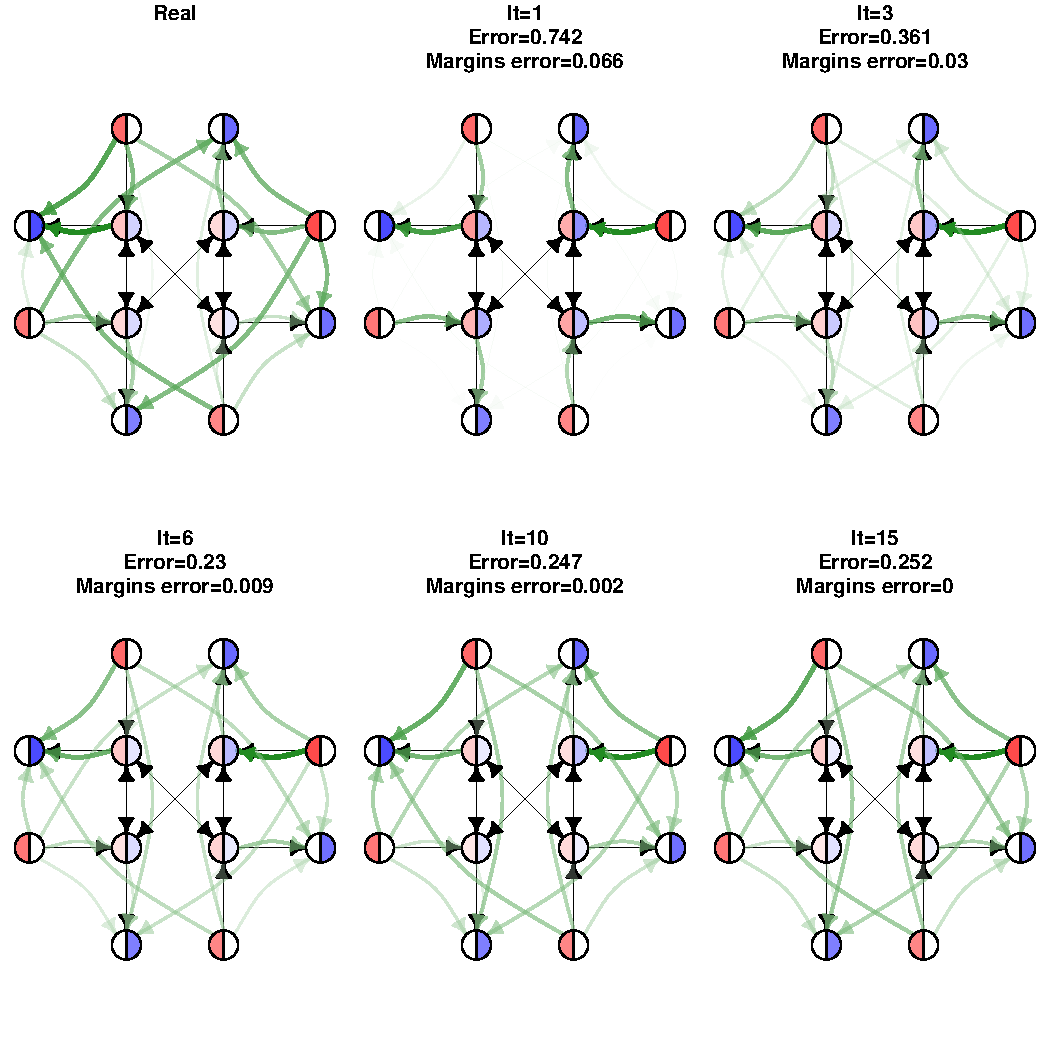
\includegraphics[width=0.98\textwidth]{fig/iterations.pdf}
	\caption{Real transportation flow (green arrows) obtained by randomly drawing $50$ passengers on the graph toy example with $p=2$ line tours, along with iterations $1, 2, 4, 7, 15$ of the algorithm with $\theta=0.001$. MTE and MME errors are computed, and embarkment and disembarkment flows are represented respectively by the red and blue colors on nodes.}
	\label{iteration_plots}
\end{figure}
On this small example, we can see that the algorithm quickly find an estimation giving small MME error, but still give an MTE of 0.256. This result is due to the fact that only $50$ passengers are drawn, giving a large deviation compared to the optimally found solution which maximize the entropy.

\subsubsection{MTE study}
\label{mte_study}

The main goal of toy examples, since we have access to the real transportation flow, is to study how the resulting $MTE$ behave regarding passenger $st$-trips distribution and hyperparameter $\theta$, on different network sizes. 

The randomness of the $st$-trips distribution is controlled by the number of drawn passengers and we can see that the algorithm performs better if this number increases, as seen in Figure \ref{MTE_vs_passengers}. This behavior can be expected as the method is constructed to find the solution maximizing the entropy while respecting embarkment and disembarkment constraint. In fact, all MTE should converge to $0$ eventually, however this rate of convergence seems to be low.
\begin{figure}[h]
	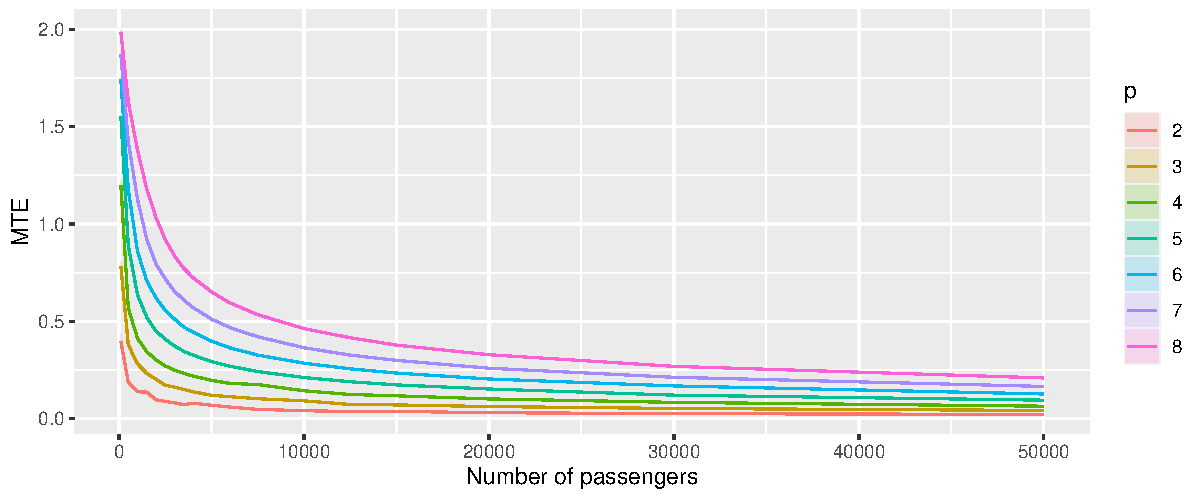
\includegraphics[width=0.98\textwidth]{fig/MTE_passengers.pdf}
	\caption{Mean transportation error (MTE) vs the number of randomly drawn passengers, in toy examples with numbers of tours $p$ varying from 2 to 8. The hyperparameter is set to $\theta=0.001$ and $10$ different draws are performed for each data point.}
	\label{MTE_vs_passengers}
\end{figure}
As for the hyperparameter study, found in Figure \ref{MTE_vs_theta}, we see that the optimal parameter seems to decreases as network size increases, reaching value close to $0$ for $8$ line tours. However, this is not the only factor which helps to decide this parameter. As a matter of fact, it seems unrealistic, in some real life scenarios, that all passengers embarking or disembarking at junctions are all transiting, and this value will be kept at $0.1$ for our real life study.
\begin{figure}[h]
	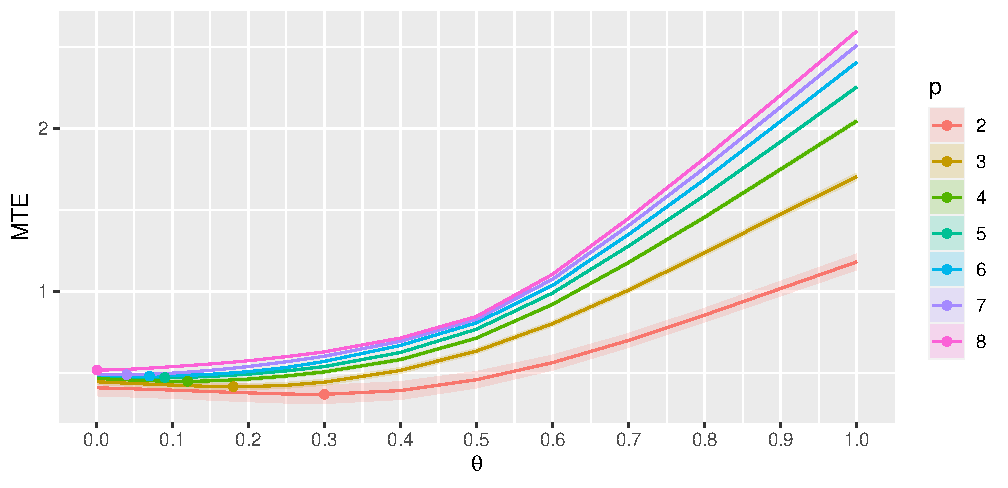
\includegraphics[width=0.98\textwidth]{fig/MTE_tours.pdf}
	\caption{Mean transportation error (MTE) vs hyperparameter $\theta$, in toy examples with numbers of tours $p$ varying from 2 to 8. The dot on each curve denotes the minimum. The number of drawn passengers is different for every network size and is set to $20 \cdot \vert P \vert$, in order to keep the randomness level constant. $10$ different draws are performed for each data point.}
	\label{MTE_vs_theta}
\end{figure}

\subsection{Real Data}
\label{real_data}

\subsubsection{The dataset and algorithm setup}
\label{data_algo}
The dataset derived from the public transportation agency in the city of Lausanne (tl), in Switzerland. Automatic passenger counters were used to collect data on the number of passengers entering and leaving buses and metros at each stop. The dataset comprises 44 lines of metro and bus transportation, 1361 stops, and over 115 million passengers per year. Each round trip forms two separate lines, which often have stops that correspond to both the inbound and outbound directions, but this is not always the case. Some stops may be unique to either the inbound or outbound direction. The initial dataset contained 13 million data rows, which were aggregated to the year 2019, and the passenger data was filtered to include only passengers who boarded and disembarked at each stop. Lines with the most errors were removed, resulting in a final dataset of 35 transportation lines and 1216 stops. The threshold for invalid lines was set when a difference of between total embarkment and disembarked differs more than 15\% of their means. For the rest all other lines, the correction found in appendix was applied to ensure consistency conditions.  

The matrix $P$, containing valid $st$-trips, was built using same condition found in toy example with an additional one. If the estimated pedestrian time (using Open Trip Planner (REF)) between two stops $s$ and $t$ was shorter than the estimated time by taking the public transportation network, this $st$-trip was also removed from $P$. The graph structure, consisting in matrices $\bm{\chi}$ and $P$, was constructed beforehand testing the method.

The algorithm was run with hyperparameter $\theta = 0.1$. Tracking the error on margins (MME) showed a rapid decreases, as seen in Figure \ref{MME_vs_iteration}, but the (conservative) convergence criterion (chosen as when $\sum_{st} \vert f^{prev}_{st} - f_{st} \vert< 10^{-6} $) was reach after 316 iterations, which corresponds to approximately one hour of computing time with a single thread.

\begin{figure}[h]
	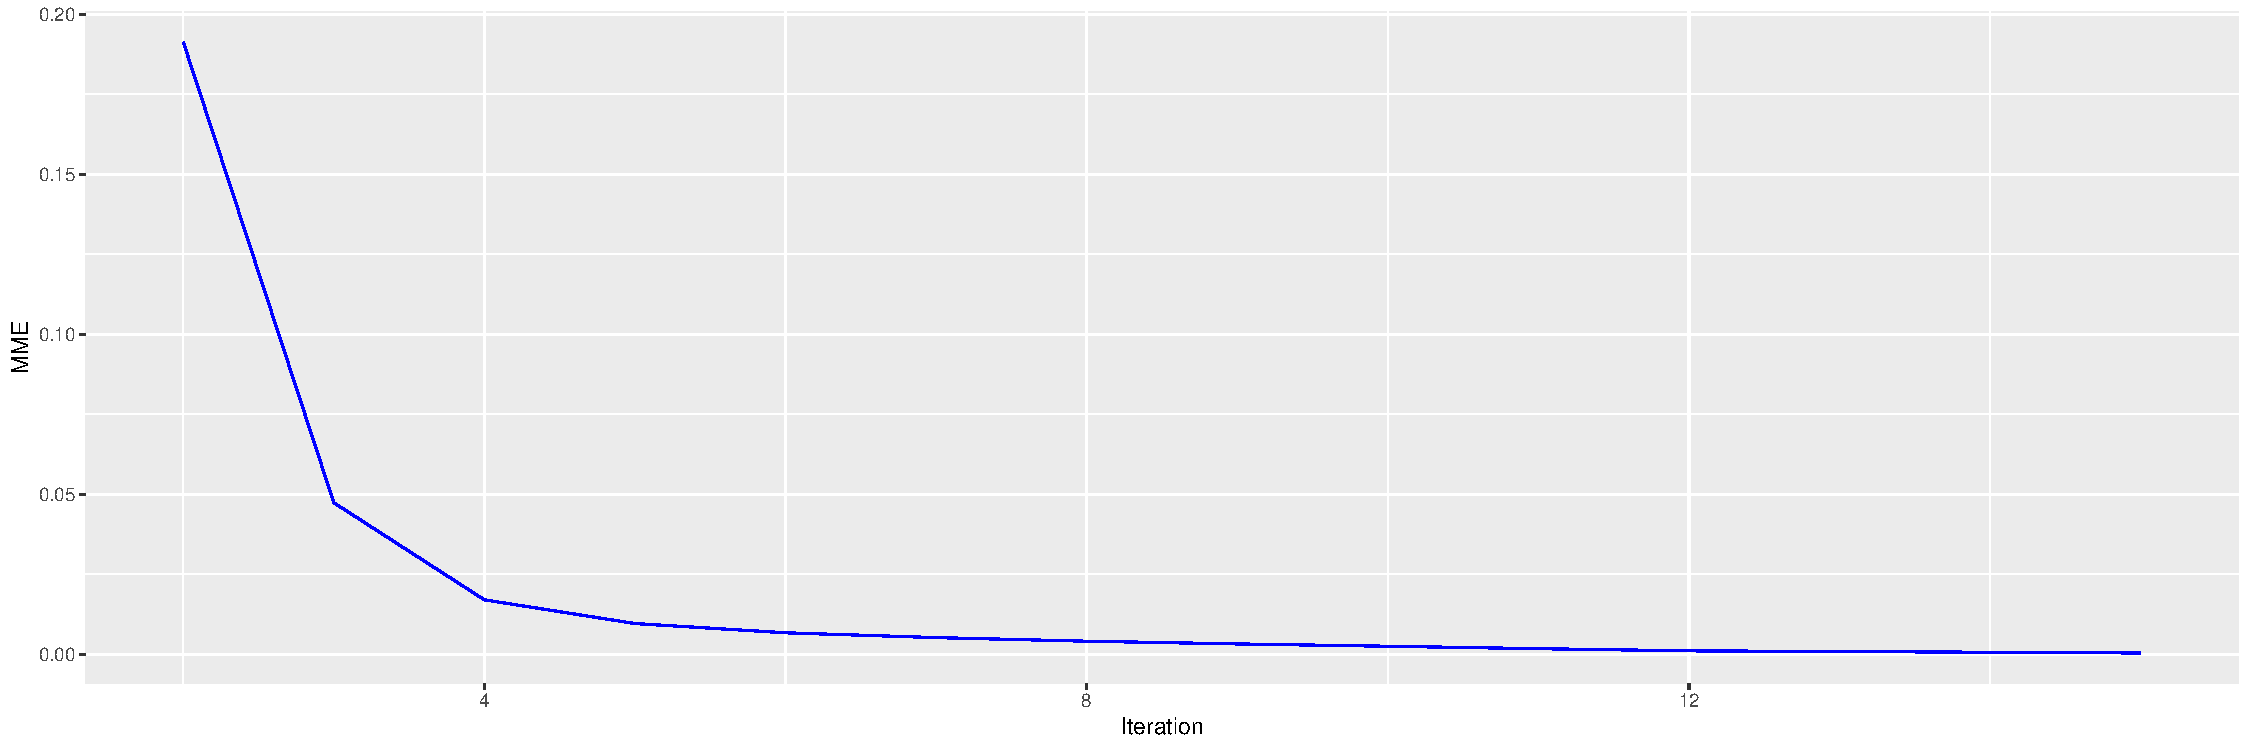
\includegraphics[width=0.98\textwidth]{fig/MME_vs_iteration.pdf}
	\caption{Mean margin error (MME) vs iteration for the algorithm run with the public transportation network data of city of Lausanne (35 lines, 1216 stops).}
	\label{MME_vs_iteration}
\end{figure}

\subsubsection{Results}
\label{lausanne_results}


%% --------------------------------- CONCLUSION

\section{Conclusion}

  
\newpage


\section*{Appendix}

\subsection*{Embarkment and disembarkment corrections for lines}
\label{flow_correction}
It may happen that, on some lines $\ell$, with stops indexed in order as $1, \ldots, l$, raw data do not obey the following necessary consistency conditions 
\begin{align*}
	a_l = 0&, \; b_1 = 0 \\
	A_{(i-1)} &\geq B_i \qquad \forall i \in \{1, \ldots, l-1\} \\
	A_{l} &= B_{l} \qquad \text{for terminal stop $l$}
\end{align*}
where $A_i$ (respectively $B_i$) is the cumulated number of embarked (resp. disembarked) passengers on the line at stop $i$. The first condition is easy to correct (by setting both quantities to $0$), and we will assume that they are valid. The last two require an iterative procedure, explained here.

We first identify all stops $i$ where $A_{i - 1} < B_i$ and store them, along with stop $1$ and $l$, in a order set $S$. Let $\text{Prev}(i)$ be the item right before $i$ in the set $S$. For all $i \in S \setminus \{1\}$, we do :
\begin{align*}
		\hat{a}_j&=\left( 1-\frac{(A_{(i-1)} - A_{(\text{Prev}(i)-1)}) - (B_{i} -  B_{\text{Prev}(i)})}{(A_{(i-1)} - A_{(\text{Prev}(i)-1)}) + (B_{i} -  B_{\text{Prev}(i)})}\right)\, a_j  \qquad \forall j \in \{ \text{Prev}(i), \ldots, i-1 \} \\
	\hat{b}_j&=\left( 1+\frac{(A_{(i-1)} - A_{(\text{Prev}(i)-1)}) - (B_{i} -  B_{\text{Prev}(i)})}{(A_{(i-1)} - A_{(\text{Prev}(i)-1)}) + (B_{i} -  B_{\text{Prev}(i)})}\right)\, b_j  \qquad \forall j \in \{ \text{Prev}(i) + 1, \ldots, i \}
\end{align*}
Before the last step, all conditions $A_{(i-1)} \geq  B_{i}$ should be respected except for node $l$. The last step ensures that $A_{l} = B_{l}$, however, as it can sometimes lower the embarkment count and increase the disembarkment count on previous nodes, some new nodes can now violate $A_{(i-1)} \geq B_i$. This is why this procedure must be iterated until all stops on the line verify consistency conditions. 

%%%%%%%%%%%%%%%%%%%%%%%%%%%%%%%%%%%%%%%%%%%%%%
%%                                          %%
%% Backmatter begins here                   %%
%%                                          %%
%%%%%%%%%%%%%%%%%%%%%%%%%%%%%%%%%%%%%%%%%%%%%%

\begin{backmatter}

\section*{Acknowledgements}%% if any
Text for this section\ldots

\section*{Competing interests}
The authors declare that they have no competing interests.

% if your bibliography is in bibtex format, use those commands:
\bibliographystyle{bmc-mathphys} % Style BST file (bmc-mathphys, vancouver, spbasic).
\bibliography{article_tl.bib}      % Bibliography file (usually '*.bib' )


\end{backmatter}
\end{document}
